\documentclass{article}

\title{Homework 1 : Graphs and Network Flows}
\author{Aashith Kamath Manjeshwar, Saikrishna Badrinarayanan}
\newcommand{\R}{\mathbf{R}}
\newcommand{\U}{\mathbf{U}}
\newcommand{\V}{\mathbf{V}}
\newcommand{\W}{\mathbf{W}}

\usepackage{graphicx}
\graphicspath{ {plots/} }
\begin{document}
\maketitle

In this project, we use the igraph library to generate different kinds of networks and measure several properties of 
each of these networks. The project was coded in the language R.

\paragraph{Problem 1}: \\
a)\\
The first problem involved creating three undirected random networks with 1000 nodes each and a probability $p$ that
every pair of nodes has an edge between them. The values of $p$ were taken as $0.01,0.05$ and $0.1$
respectively for each of the three graphs. After this, we plot the degree distribution for each of the graphs.
The degree distribution is a plot containing the various degrees of the nodes in the graph on the x-axis
and their corresponding density (frequency of that degree occuring divided by the total number of nodes) on the y-axis.\\

The degree distribution plot for the first graph is :\\
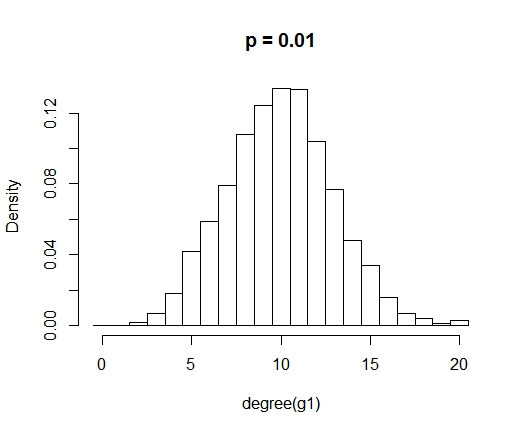
\includegraphics[scale=0.4]{pa1} \\
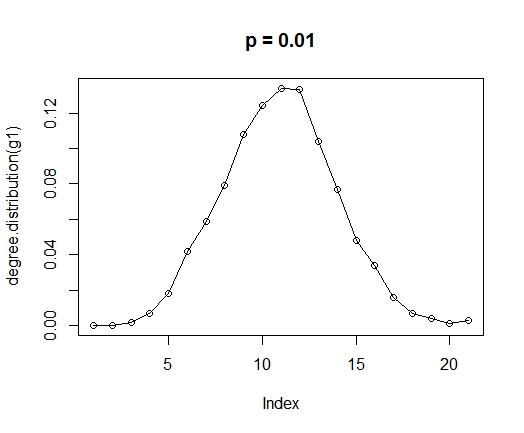
\includegraphics[scale=0.4]{pa2} \\
The degree distribution plot for the second graph is :\\
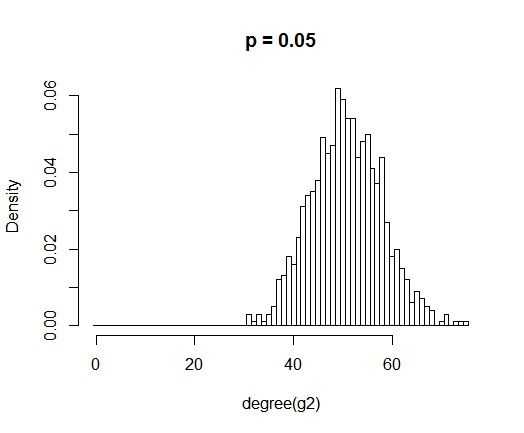
\includegraphics[scale=0.4]{pa5} \\
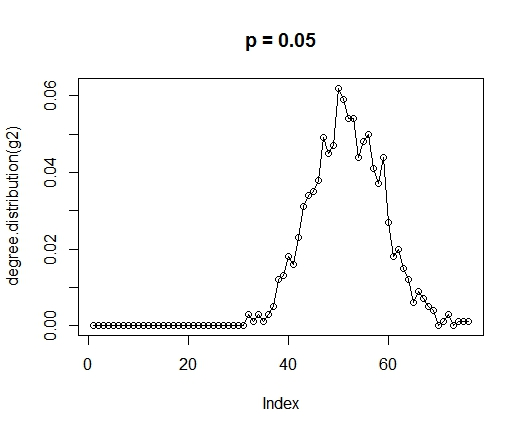
\includegraphics[scale=0.4]{pa6} \\
The degree distribution plot for the third graph is :\\
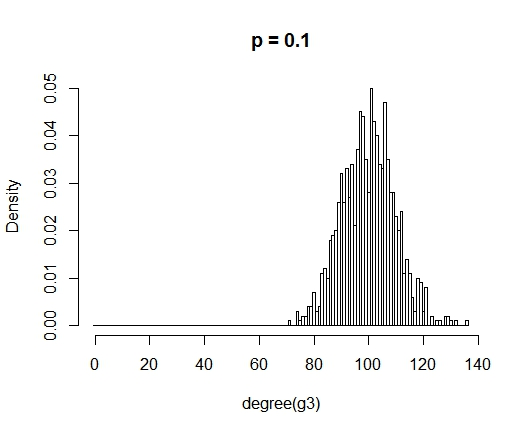
\includegraphics[scale=0.4]{pa9} \\
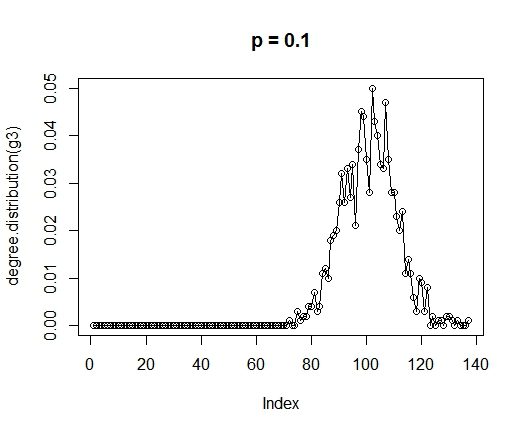
\includegraphics[scale=0.4]{pa10} \\
After this, we repeated the same process above 100 times and plot the average degree distribution over the 100 random 
graphs below.\\

The average degree distribution for $p=0.01$ is \\
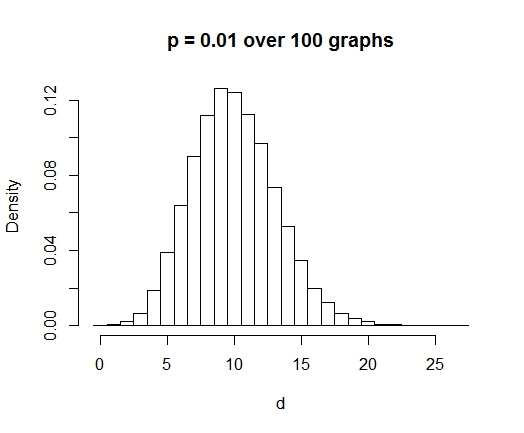
\includegraphics[scale=0.4]{pa3} \\
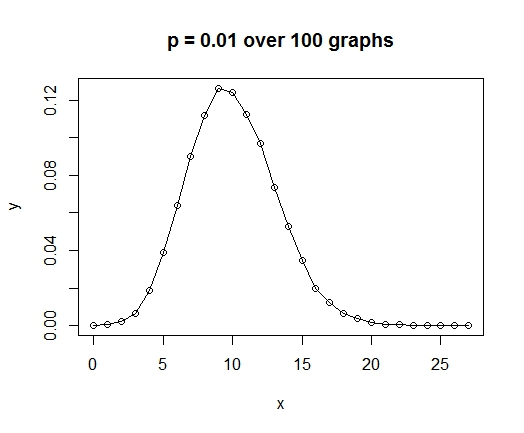
\includegraphics[scale=0.4]{pa4} \\
The average degree distribution for $p=0.05$ is \\
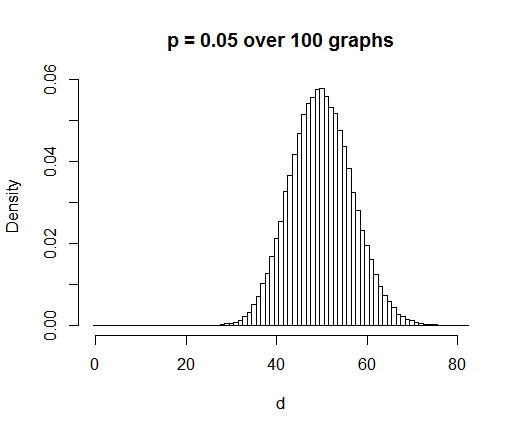
\includegraphics[scale=0.4]{pa7} \\
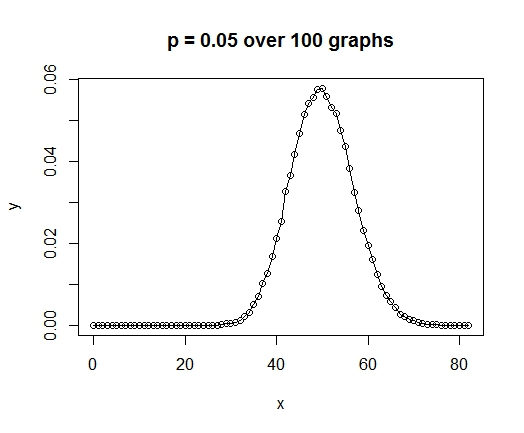
\includegraphics[scale=0.4]{pa8} \\
The average degree distribution for $p=0.1$ is \\
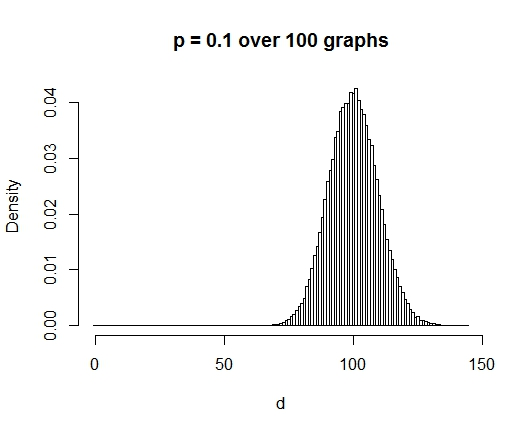
\includegraphics[scale=0.4]{pa11} \\
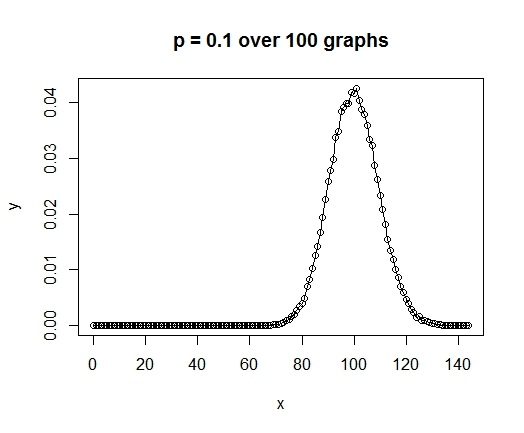
\includegraphics[scale=0.4]{pa12} \\
b)\\
This question asks whether the graphs generated above are connected or disconnected and to find out their diameters.
In the rest of the question, let's denote the graph generated with $p=0.01$ as the first graph,
$p=0.05$ as the second graph and $p=0.1$ as the third graph. The diameter of a graph is the length of the shortest path 
between the nodes with the longest distance between them. That is, the length of the shortest path between the nodes
that are farthest apart.
\begin{itemize}
 \item 
 The first graph is connected and it's diameter is 6.
 \item
 The second graph is connected and it's diameter is 3.
 \item
 The third graph is connected and it's diameter is 3.
\end{itemize}

c)\\
In this question, the aim is to numerically find a value $p_c$ such that when $p<p_c$, the random networks we 
generate (with probability of every pair of nodes having an edge being $p$) is disconnected and when 
$p>p_c$, the generated random networks are connected. The way we do this is that we generate a random graph and 
check for different values of $p$ whether the graph is connected or not. We thus obtain a minimum and maximum value of 
$p_c$, i.e beyond the maximum value, for all $p$, the graph is connected and below the minimum value,
for all $p$, the graph is disconnected.\\
We note that since the graphs generated are random, the minimum and maximum values of $p_c$ will change (slightly)
if we run the procedure again. As a result, we repeat the process 100 times and take the average values.
We observe that, after averaging, the minimum value of $p_c$ is $0.0054$ and the maximum value is $0.0072$.\\
If we are required to give exactly 1 value of $p_c$ such that the graph is disconnected for all $p<p_c$ and connected
for all $p>p_c$, we can average the minimum and maximum values to obtain $p_c=0.0063$\\

d)\\
In this question, we are expected to analytically calculate the value of $p_c$.\\
Let's first calculate the probability that a given node $i$ is isolated. For a given node $i$, it is isolated only if
it has no edges with any other nodes. The probability of it not having an edge with another particular node $j$ is 
$(1-p)$. Since the probability that $i$ has an edge with any chosen node is exactly $p$ and is independent of whether it
has edges with other nodes, the probability that $i$ has no edges with $(1-p)^n$. Thus, the probability that a given 
node is isolated is $(1-p)^n$. Since we expect the value of $p$ to be small (i.e 
when $p=p_c$ we expect it to be small as for higher values of $p$, it's unlikely that the graph is disconnected),
we can approximate $(1-p)^n$ to $e^{-pn}$.\\
Now, let's calculate how many nodes are isolated. Rather, we will compute the expectation of the number of isolates nodes. 
Let's denote this quantity by $E(x)$.\\
If the graph has $n$ verticies $v_1,\ldots v_n$, we can write $E(x) = E(x_1) + E(x_2) + \ldots E(x_n)$, where
$E(x_i)$ is the expectation that vertex $v_i$ is isolated. From our earlier calculation, 
$E(x_i) = 1.e^{-pn} + 0.(1- e^{-pn}) = e^{-pn}$ $\forall i$. \\
Thus, $E(x) = n.e^{-pn}$\\

We note that if $E(x)>=1$, it means that the expected number of isolated nodes is 
atleast 1 and so the graph must be disconnected. However, if $E(x) <1$, it just means that the expected number of isolated nodes
is less than 1. The graph could still be disconnected in such a case. For example, a simple graph with 4 vertices in which
the first two vertices have an edge between them, the third and fourth vertices have an edge between them. The graph is
disconnected but no vertex is isolated. However, since we know that if $E(x)>=1$, the graph is surely disconnected,
we will use this measure to determine our value of $p_c$.\\
$E(x)>=1 \Rightarrow n.e^{-pn} >=1 $\\
$\Rightarrow n>= e^{pn} \Rightarrow ln(n) >=pn $\\
$\Rightarrow p<=ln(n)/n$\\
Thus, whenever $p<=ln(n)/n$, the graph is disconnected. Hence the value of $p_c$ is $ln(n)/n$.\\

For $n=1000$, $ln(n)/n = 0.0069$. Thus, we observe that the numerically computed value in the previous question 
roughly matches with the analytically computed one for $n=1000$.\\

\hrule
\paragraph{2)}
a)\\
This problem involves creating an undirected random network with 1000 nodes whose degree 
distribution is proportional to $x^{-3}$ (a fat-tailed degree distribution).
The degree distribution is a plot containing the various degrees of the nodes in the graph on the x-axis
and their corresponding density (frequency of that degree occuring divided by the total number of nodes) on the y-axis.\\
We use the barabasi-albert model to generate the graph.\\
The degree distribution plot for the graph is :\\
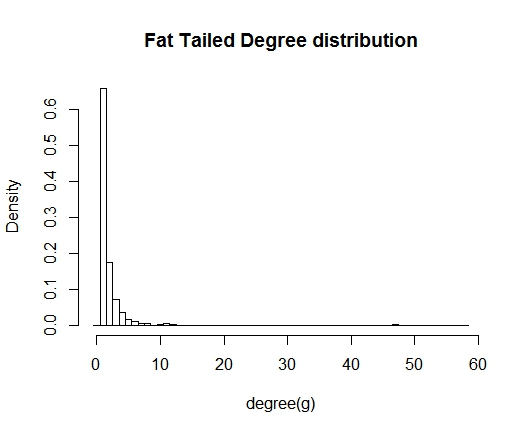
\includegraphics[scale=0.4]{pb1} \\
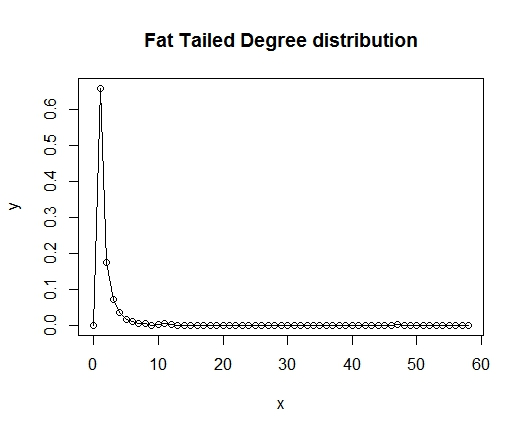
\includegraphics[scale=0.4]{pb2} \\
After that, we compute the diameter of the graph and it turns out to be 16.\\

b)\\
In this question, we first check if the graph is connected and it turns out that it indeed is.\\
We then find the Giant Connected Component (GCC). The GCC of a graph is a connected component that 
contains a constant fraction of the entire graph's vertices.
We find the GCC by first computing the set of clusters in the graph
and then the largest cluster among them. We then delete the vertices that do not belong to the largest cluster and this gives
the GCC. We then plot the degree distribution of the GCC and it is shown below.\\
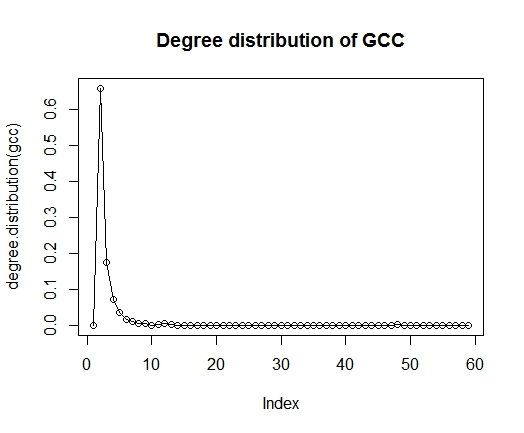
\includegraphics[scale=0.4]{pb3} \\

We then find the community structure using the fast greedy method on the GCC. 
A network is said to have a community structure if the nodes of the network 
can be easily grouped into (potentially overlapping) sets of nodes such that each set is densely connected internally. 
The community structure is :\\
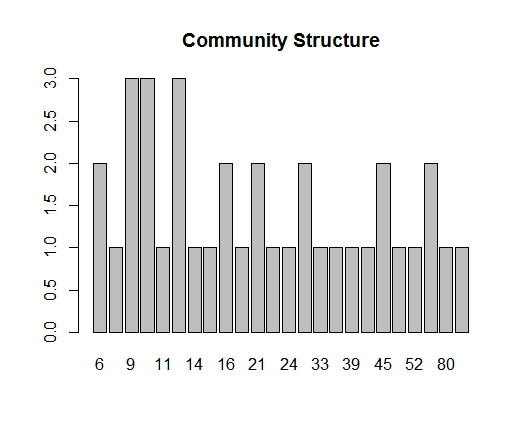
\includegraphics[scale=0.4]{pb4} \\

We then compute the modularity of the graph and it turns out to be $0.9184294$\\
The modularity is so large because there is good connectivity within the modules and not very good community 
between the modules in the graph.\\

c)\\
In this problem, we create a larger network with $10000$ nodes whose degree distribution is proportional to $x^-3$.
We then compute the GCC and the community structure as in the previous question. The community structure is :\\
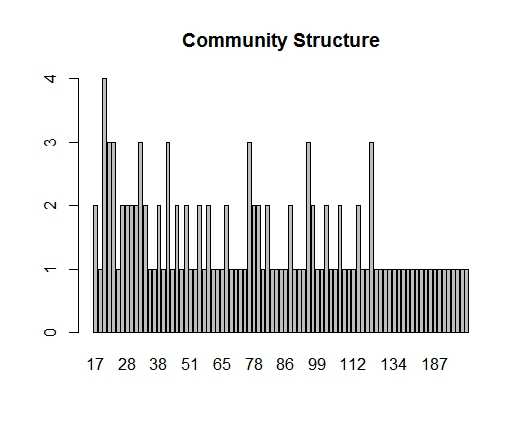
\includegraphics[scale=0.4]{pb5}\\.
After this, we measure the modularity of this graph and it turns out to be $0.9760596$ which is larger than that
in the case of the smaller graph.\\

d)\\
Here, we first randomly pick a node $i$ and then randomly pick one of it's neighbours $j$. We repeat this process 
$100000$ times and plot the degree distribution of the nodes $j$ picked in this process. The degree distribution is :\\
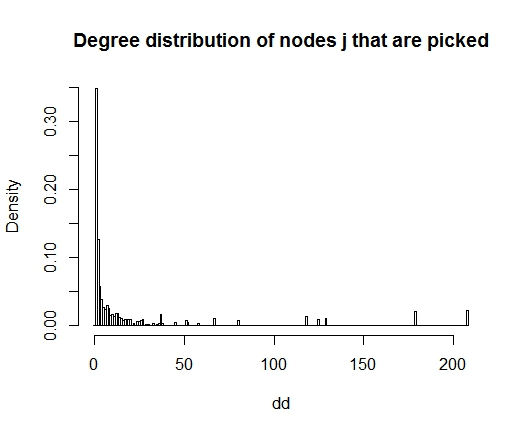
\includegraphics[scale=0.4]{pb6} \\
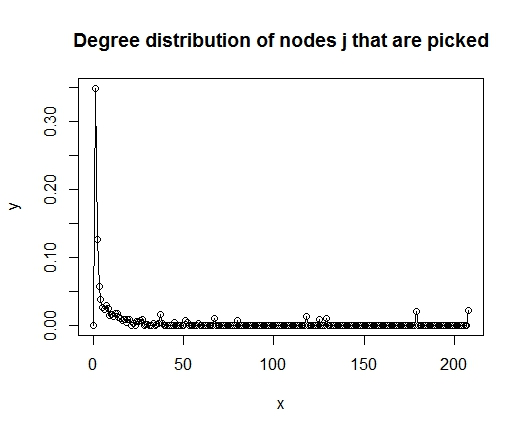
\includegraphics[scale=0.4]{pb7} \\

\hrule

\paragraph{3)}
a)\\
In this problem, we create an undirected graph by simulating it's evolution.
Each time a new vertex is added it creates a number of new links
to old vertices and the probability that an old vertex is cited (included in the graph)
depends on its in-degree and age. This process of adding the old vertex depending on it's 
high in-degree and age is called preferential attachment. We create such an undirected network with 1000 nodes
and plot it's degree distribution \\
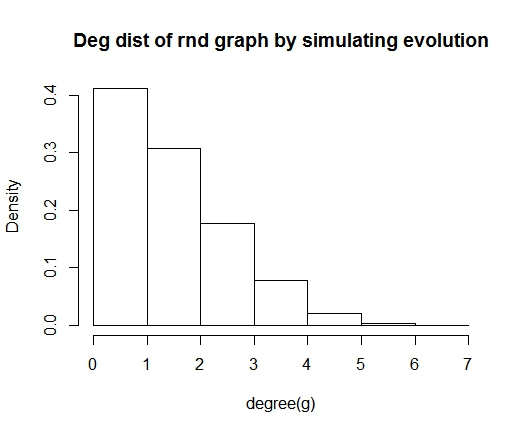
\includegraphics[scale=0.4]{pc1} \\
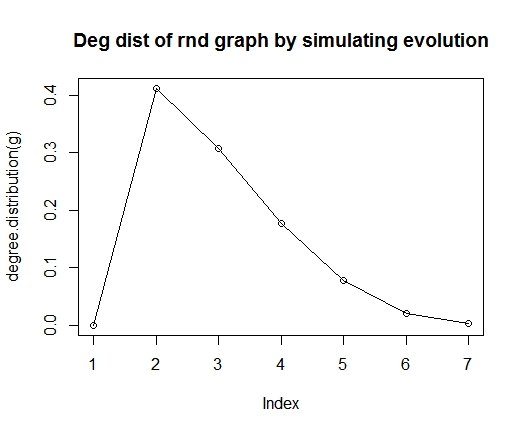
\includegraphics[scale=0.4]{pc2} \\

After this, we repeated the same process above 100 times and plot the average degree distribution over the 100 random 
graphs below.\\

The average degree distribution is \\
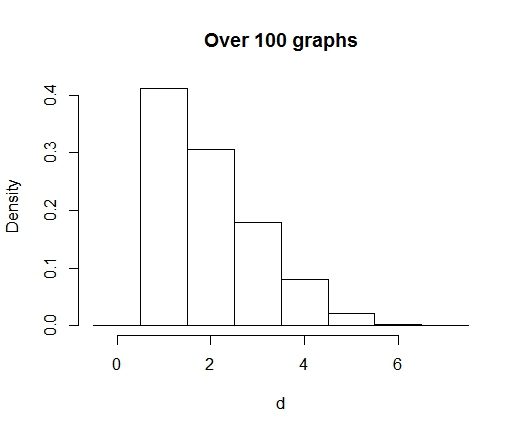
\includegraphics[scale=0.4]{pc3} \\
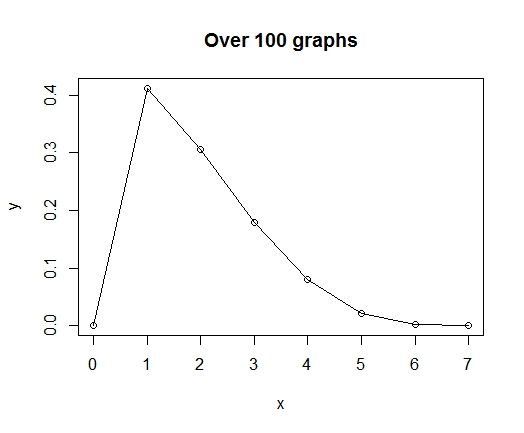
\includegraphics[scale=0.4]{pc4} \\

b)\\
As in problem 2, we find the GCC and use fast greedy method to compute the community structure. The community structure is :\\
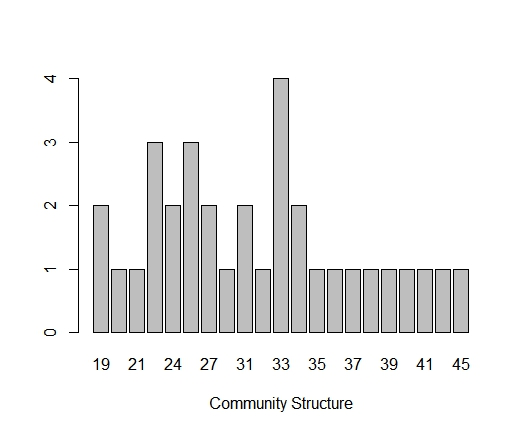
\includegraphics[scale=0.4]{pc5} \\
We then measure the modularity and it is equal to $0.9359986$.\\

\hrule

\paragraph{4)}
a)\\
In this problem, we create a graph by using the forest fire model.
This is a growing network model, which resembles how the
forest fire spreads by igniting trees close by. Unlike previous cases, it is a directed graph.
We create several graphs with the forward burning probability ranging from $0.1$ to $0.4$
and the backward burning ratio set as $1$.
We then plot the in and out degree distributions. We define graph 1 as the one with forward burning probability 
as $0.1$, graph 2 with $0.2$, graph 3 with $0.27$ and graph 4 with $0.37$. Apart from the normal in-degree and out-degree plots,
we additionally draw one more plot for each graph. We plot the density vs degree on a log log scale with both the in and out 
degrees. The ``triangles'' in the graph are for the out-degree and the ``circles'' are for the in-degree.\\
\textbf{Graph 1}\\
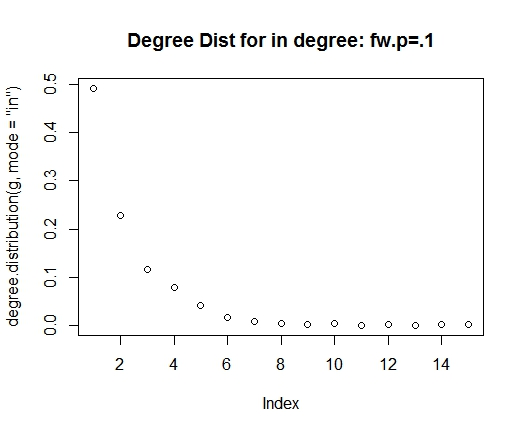
\includegraphics[scale=0.4]{pd1} \\
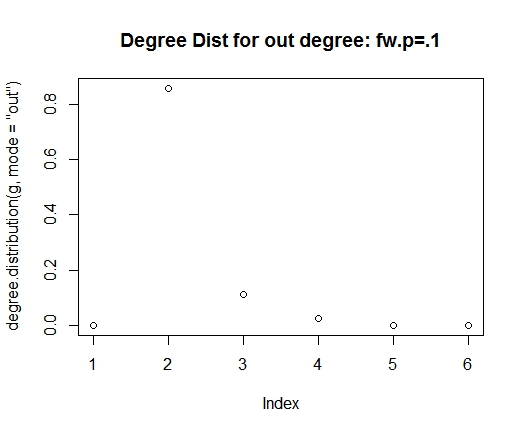
\includegraphics[scale=0.4]{pd2} \\
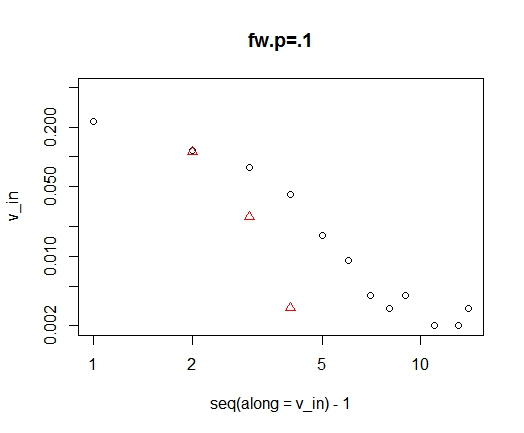
\includegraphics[scale=0.4]{pd5} \\
\textbf{Graph 2}\\
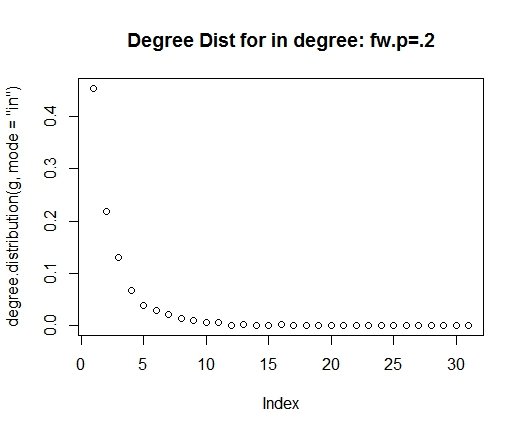
\includegraphics[scale=0.4]{pd6} \\
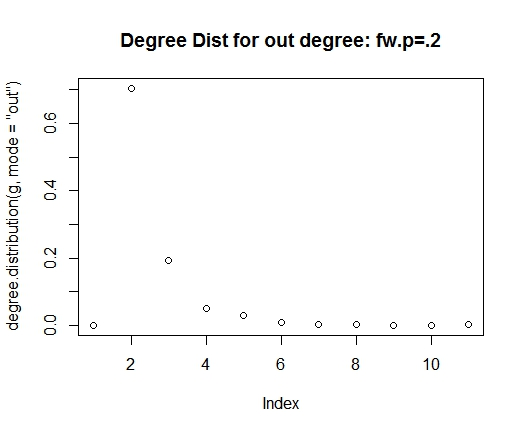
\includegraphics[scale=0.4]{pd7} \\
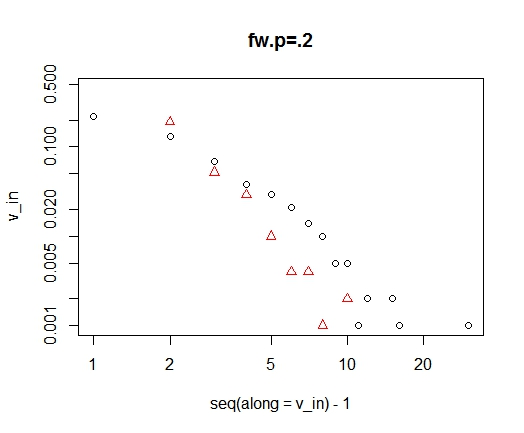
\includegraphics[scale=0.4]{pd10} \\
\textbf{Graph 3}\\
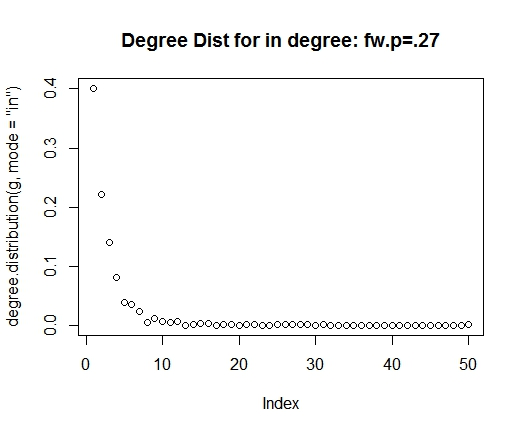
\includegraphics[scale=0.4]{pd11} \\
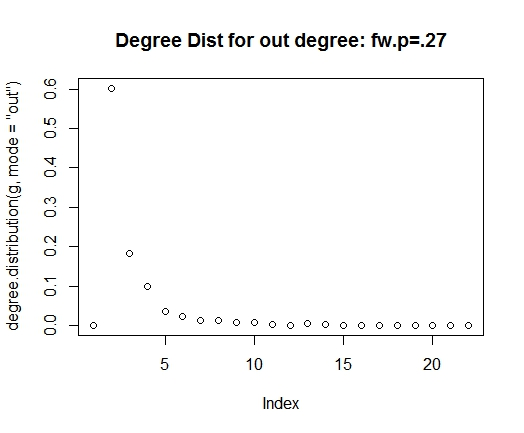
\includegraphics[scale=0.4]{pd12} \\
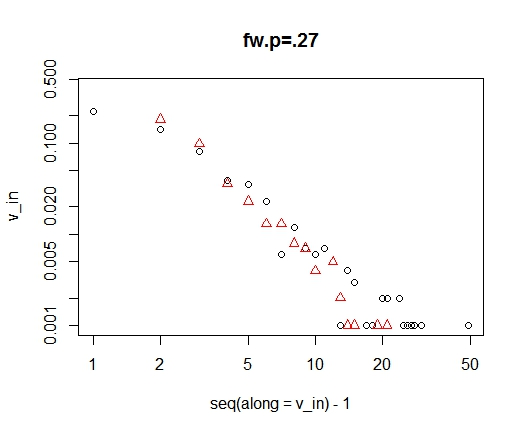
\includegraphics[scale=0.4]{pd15} \\
\textbf{Graph 4}\\
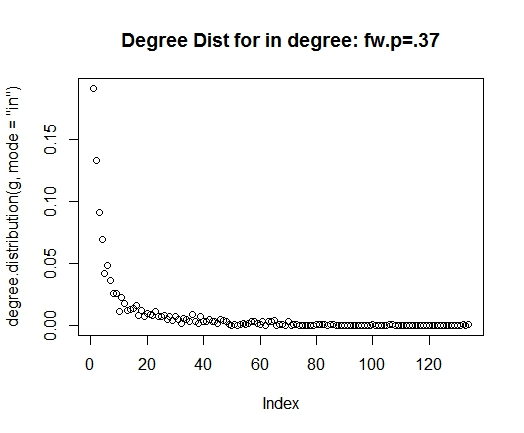
\includegraphics[scale=0.4]{pd16} \\
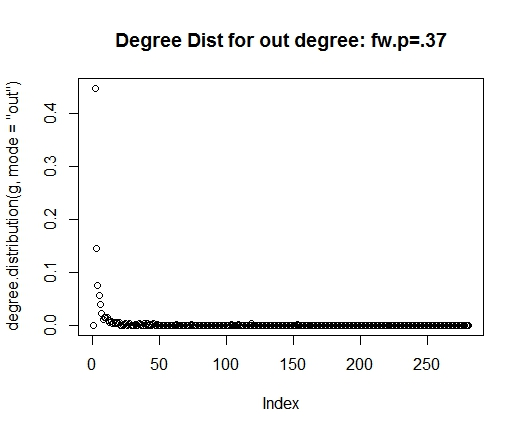
\includegraphics[scale=0.4]{pd17} \\
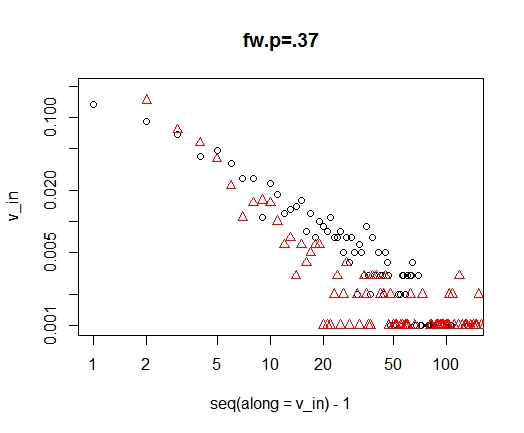
\includegraphics[scale=0.4]{pd20} \\
b)\\
We measure the diameters of the $4$ graphs.\\
\begin{itemize}
 \item 
 Graph 1 : Diameter is 14.
 \item 
 Graph 2 : Diameter is 15.
 \item 
 Graph 3 : Diameter is 10.
 \item 
 Graph 4 : Diameter is 12.
\end{itemize}

c)\\
In this problem, we find the community stucture of the 4 graphs. We use two approaches to do this.\\

In the first approach, since the fast greedy method only works on undirected graphs, we convert
the directed GCC into an undirected one using the ``as.indirected'' function with the mode being ``collapse''
the igraph library. This converts the directed graph by creating one undirected edge for each pair of vertices which are 
connected with atleast one directed edge. It doesn't create multiple edges. There are other modes like ``each'' and ``mutual''
but we choose to work with the ``collapse'' mode (for no particular reason).\\

The community structure of the first graph is :\\
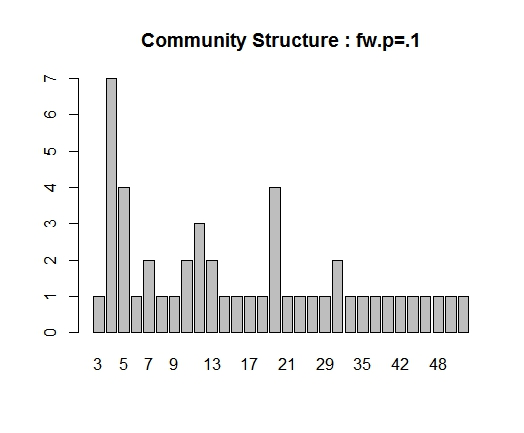
\includegraphics[scale=0.4]{pd3} \\
The community structure of the second graph is :\\
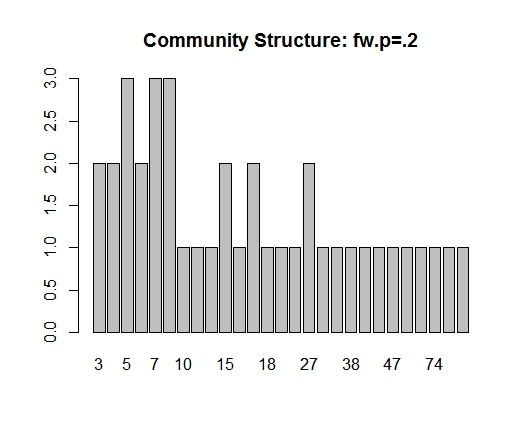
\includegraphics[scale=0.4]{pd8} \\
The community structure of the third graph is :\\
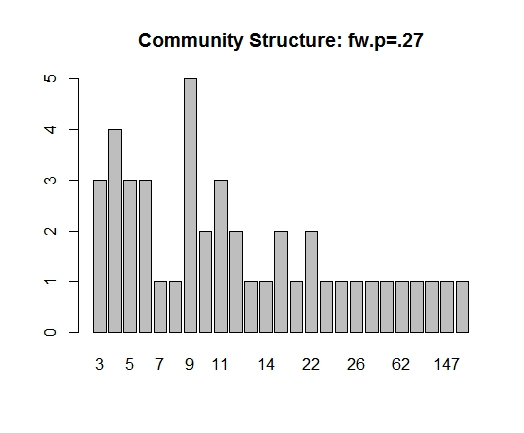
\includegraphics[scale=0.4]{pd13} \\
The community structure of the fourth graph is :\\
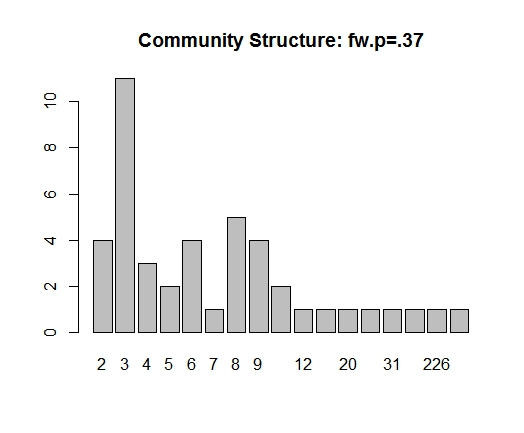
\includegraphics[scale=0.4]{pd18} \\
We then compute the modularity of the 4 graphs.\\
\begin{itemize}
 \item 
 Graph 1 : modularity is $0.9045291$
 \item 
 Graph 2 : modularity is $0.8848962$
 \item 
 Graph 3 : modularity is $0.7781591$
 \item 
 Graph 4 : modularity is $0.2152621$
\end{itemize}

In the next approach, we find the community structure by using the ``edge.betweenness.community'' function on the directed 
GCC and then find the modularity as in the previous case.\\
The community structure of the first graph is :\\
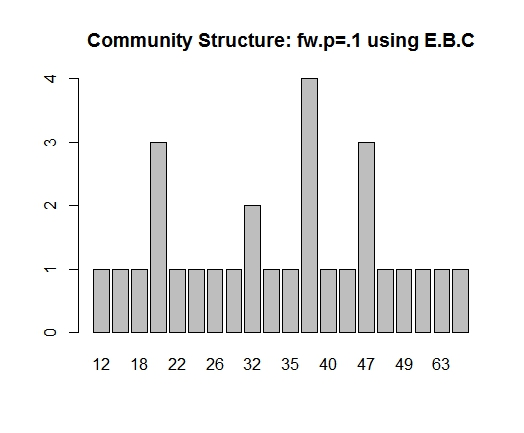
\includegraphics[scale=0.4]{pd4} \\
The community structure of the second graph is :\\
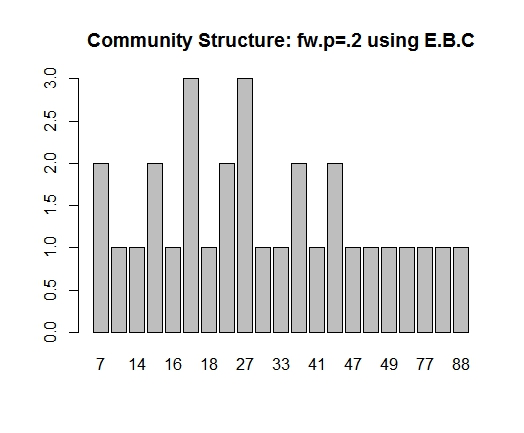
\includegraphics[scale=0.4]{pd9} \\
The community structure of the third graph is :\\
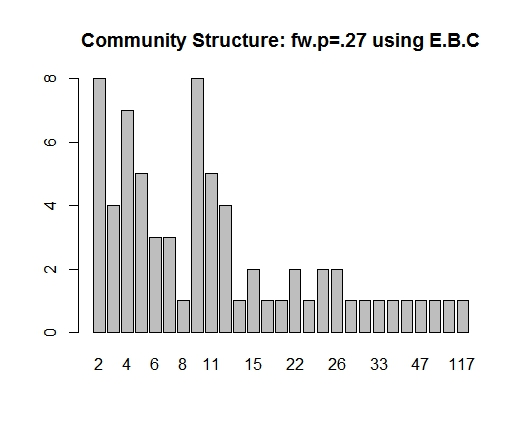
\includegraphics[scale=0.4]{pd14} \\
The community structure of the fourth graph is :\\
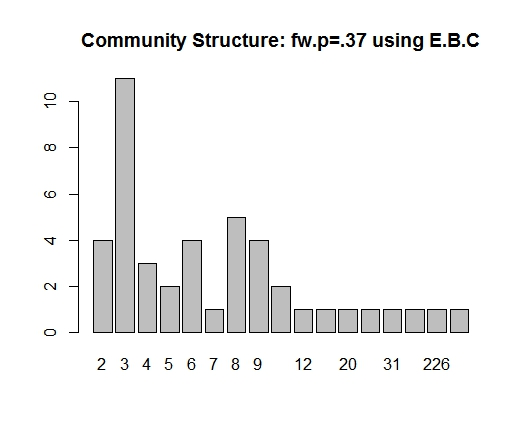
\includegraphics[scale=0.4]{pd19} \\
We then compute the modularity of the 4 graphs.\\
\begin{itemize}
 \item 
 Graph 1 : modularity is $0.9179842$
 \item 
 Graph 2 : modularity is $0.8978998$
 \item 
 Graph 3 : modularity is $0.7766938$
 \item 
 Graph 4 : modularity is $0.07439451$
\end{itemize}
We conclude by noting that both the approaches seem to give roughly the same results with a few minor differences.
\end{document}
